% govsmart_fig3.tex — Standalone status-comprehension bar chart for GovSmart paper
% Horizontal stacked bars showing correct / partly correct / incorrect per status
% Compile: pdflatex govsmart_fig3.tex
\documentclass[border=4pt]{standalone}
\usepackage[T1]{fontenc}
\usepackage{pgfplots}
\pgfplotsset{compat=1.18}
\usepackage{xcolor}

\definecolor{cCorr}{HTML}{2E7D32}    % Correct — green
\definecolor{cPart}{HTML}{F9A825}    % Partly correct — amber
\definecolor{cInc}{HTML}{C62828}     % Incorrect — red
\definecolor{cAnnot}{HTML}{E65100}   % Annotation colour

\begin{document}
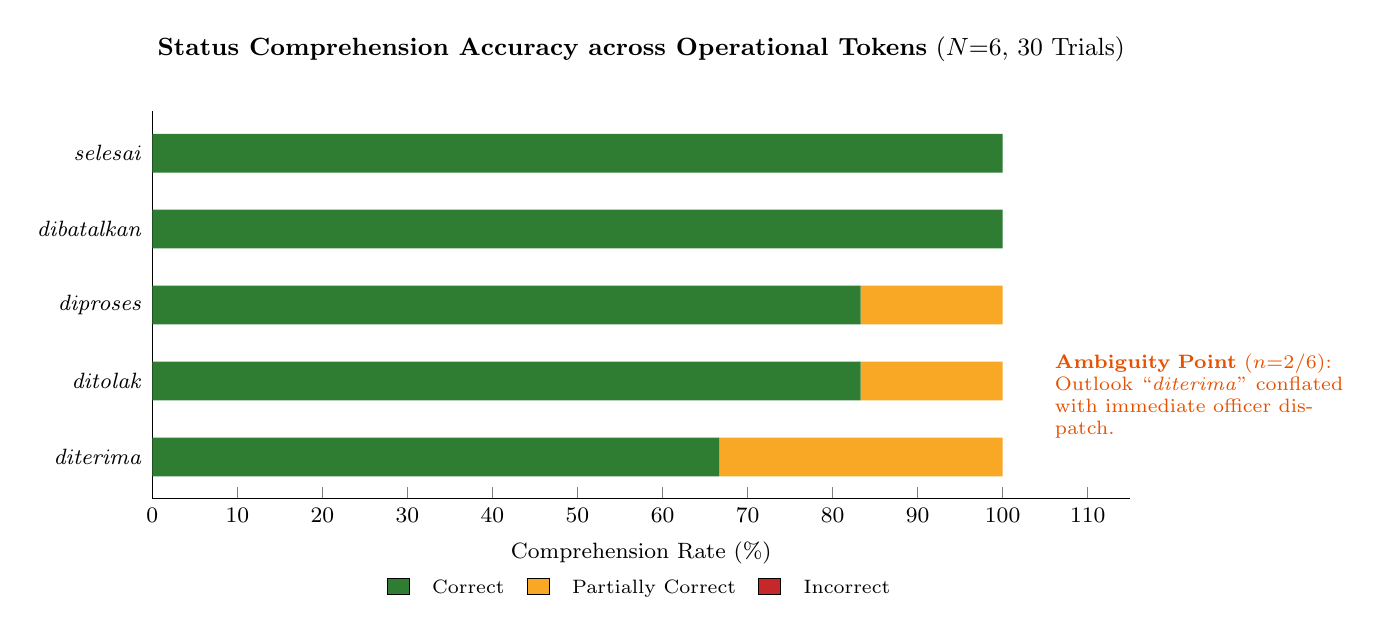
\begin{tikzpicture}
\begin{axis}[
    title={\textbf{Status Comprehension Accuracy across Operational Tokens} ($N{=}6$, 30 Trials)},
    title style={font=\small, at={(0.5,1.06)}, anchor=south},
    xbar stacked,
    width=14cm, height=6.5cm,
    bar width=14pt,
    xmin=0, xmax=115,
    xlabel={Comprehension Rate (\%)},
    xlabel style={font=\footnotesize},
    ytick={1,2,3,4,5},
    yticklabels={\textit{diterima}, \textit{ditolak}, \textit{diproses}, \textit{dibatalkan}, \textit{selesai}},
    yticklabel style={font=\footnotesize, anchor=east},
    tick label style={font=\footnotesize},
    legend style={
        at={(0.5,-0.18)},
        anchor=north,
        legend columns=3,
        font=\scriptsize,
        draw=none,
        column sep=6pt,
    },
    enlarge y limits={abs=0.55},
    axis lines*=left,
    clip=false,
]

% Correct
\addplot[fill=cCorr, draw=none] coordinates {
    (100,5) (100,4) (83.3,3) (83.3,2) (66.7,1)
};
% Partly correct
\addplot[fill=cPart, draw=none] coordinates {
    (0,5) (0,4) (16.7,3) (16.7,2) (33.3,1)
};
% Incorrect
\addplot[fill=cInc, draw=none] coordinates {
    (0,5) (0,4) (0,3) (0,2) (0,1)
};

% Percentage labels
\node[font=\scriptsize, white] at (axis cs:50,5) {100};
\node[font=\scriptsize, white] at (axis cs:50,4) {100};
\node[font=\scriptsize, white] at (axis cs:41.7,3) {83.3};
\node[font=\scriptsize, white] at (axis cs:41.7,2) {83.3};
\node[font=\scriptsize, white] at (axis cs:33.3,1) {66.7};

% Partly-correct labels (only where nonzero)
\node[font=\scriptsize] at (axis cs:91.7,3) {16.7};
\node[font=\scriptsize] at (axis cs:91.7,2) {16.7};
\node[font=\scriptsize] at (axis cs:83.3,1) {33.3};

% Ambiguity annotation — callout placed to the right, well clear of bars
\node[font=\scriptsize, cAnnot, text width=3.8cm, align=left, anchor=west]
    at (axis cs:105,1.8) {%
        \textbf{Ambiguity Point} ($n{=}2/6$):\\
        Outlook ``\textit{diterima}'' conflated\\
        with immediate officer dispatch.};

\legend{Correct, Partially Correct, Incorrect}
\end{axis}
\end{tikzpicture}
\end{document}
